\section{开发问题集锦}
\subsection{链接错误}
\subsubsection{以太网 \lstinline{Task} 代码段未明确存放位置}
仅添加以太网 \lstinline{Task} 及 \lstinline{SWC} 后,编译链接时,报错误见图 \ref{fig:ld_error_eth_task}:

\begin{figure}[htbp]
    \centering
    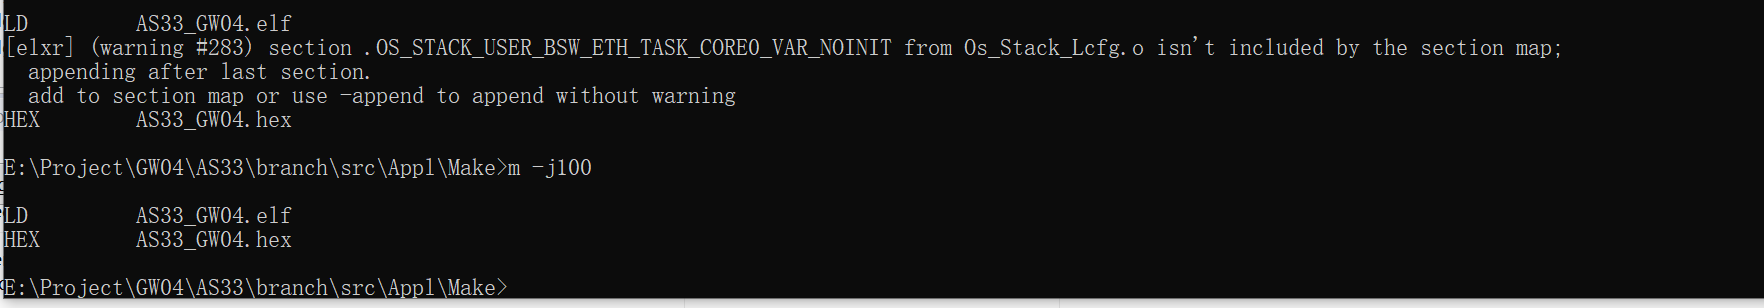
\includegraphics[scale=0.6]{pic/eth_ld_error_task.png}
    \caption{以太网 Task 代码段链接错误}
    \label{fig:ld_error_eth_task}
\end{figure}

添加新的\lstinline{Task}后,需要重新生成 \lstinline{rte os vlinkgen} 等模块。\lstinline{vlinkgen} 未生成时,报上述错误。

重要的新增生成内容如图 \ref{fig:add_task_generate_mode_code}:由于全局的 \lstinline{memmap} 文件内容修改,所以需要重新编译的文件比较多。

\begin{figure}[htbp]
    \centering
    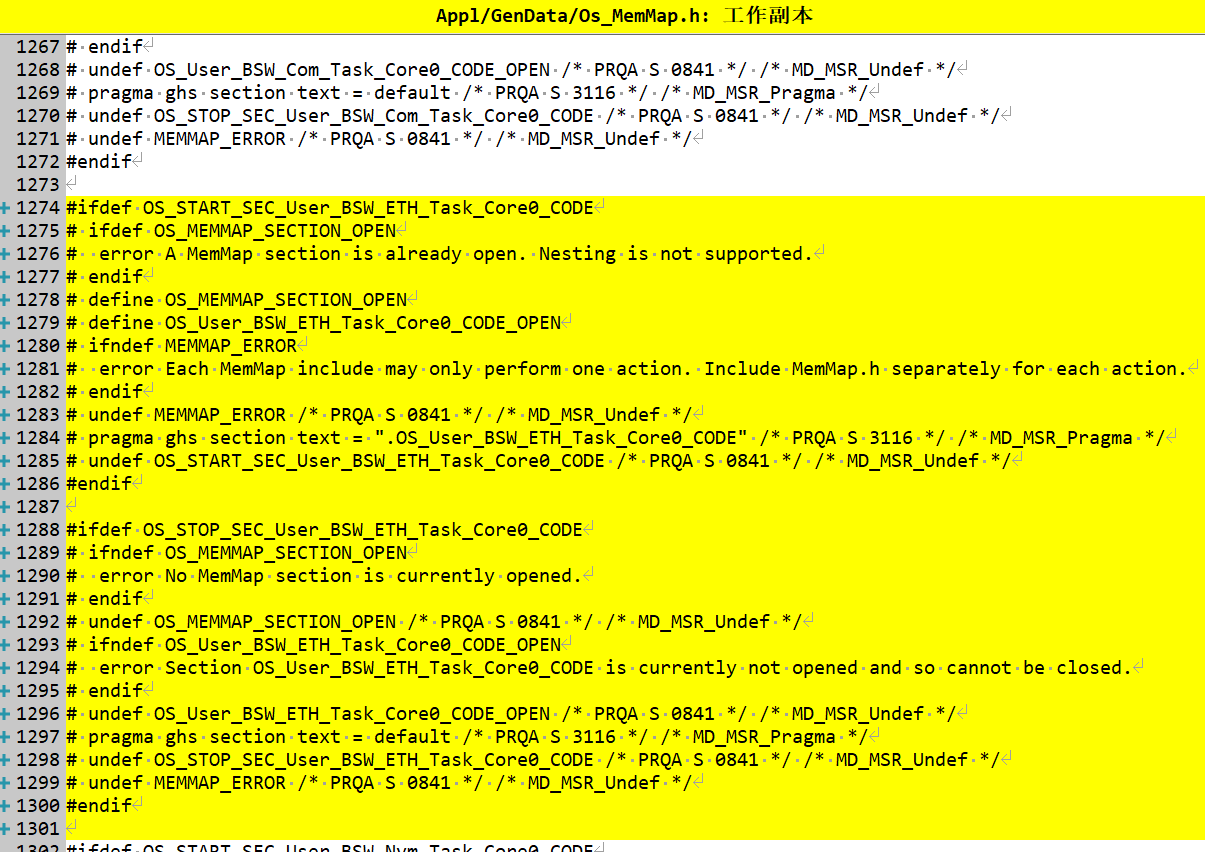
\includegraphics[scale=0.6]{pic/add_task_generate_mode_code_1.png}
    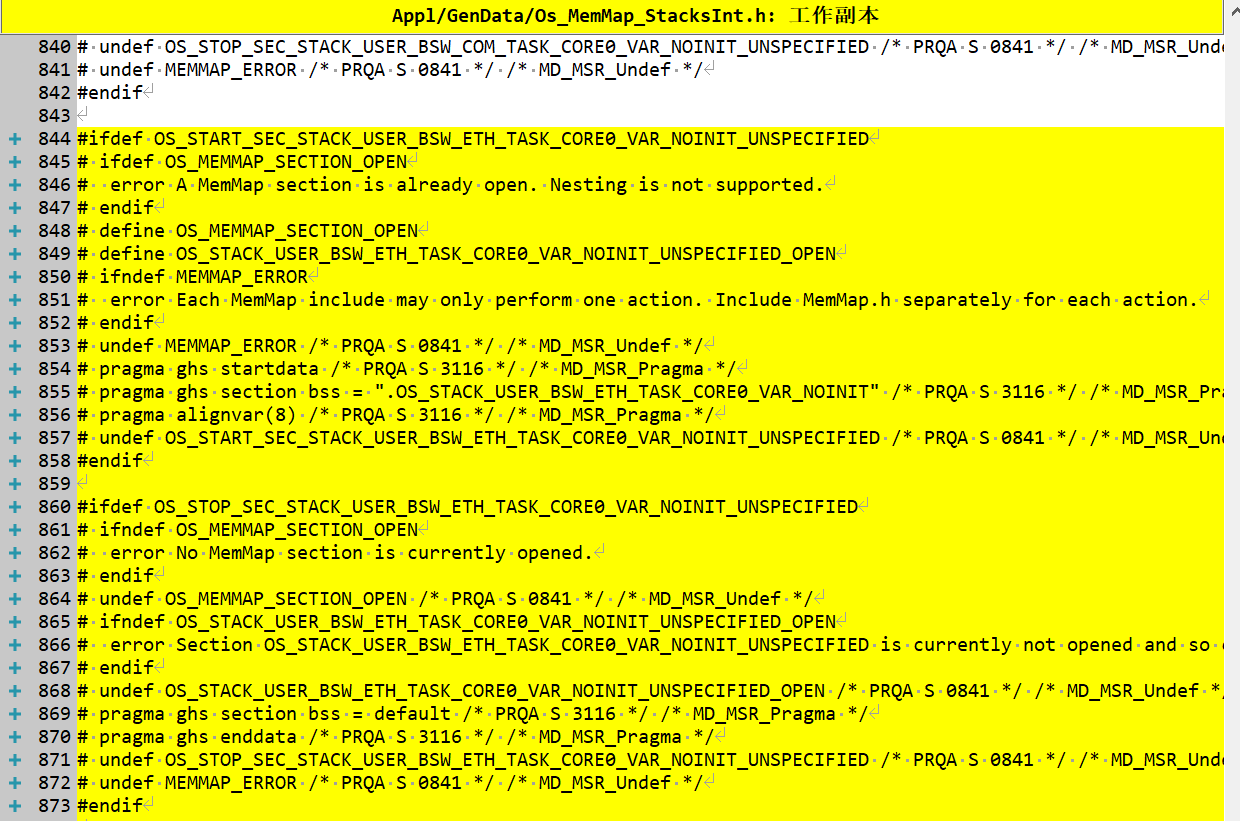
\includegraphics[scale=0.6]{pic/add_task_generate_mode_code_2.png}
    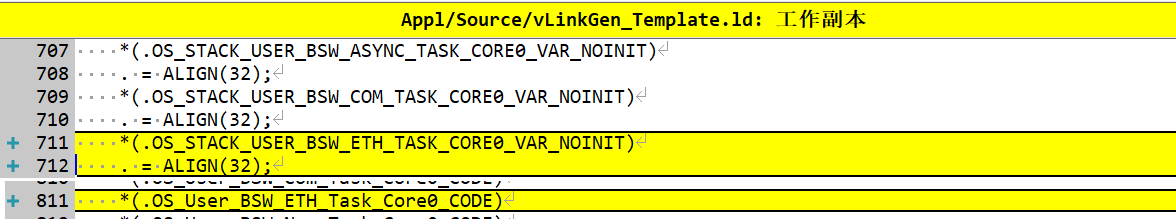
\includegraphics[scale=0.6]{pic/add_task_generate_mode_code_3.png}
    \caption{添加一个 ETH TASK 后,改变的代码}
    \label{fig:add_task_generate_mode_code}
\end{figure}

\subsubsection{添加以太网中断后 \lstinline{interrupts_flash flash} 块大小溢出}

由于对齐大小的限制,在添加以太网功能后,由于新增两个中断(\lstinline{RX TX}),导致存放中断向量表和异常向量表的 \lstinline{interrupts_flash flash} 块大小超出链接文件的大小限制。
报图 \ref{fig:eth_ld_error_interrupts_flash_overflow} 错误。此错误在链接阶段报出。

\begin{figure}[htbp]
    \centering
    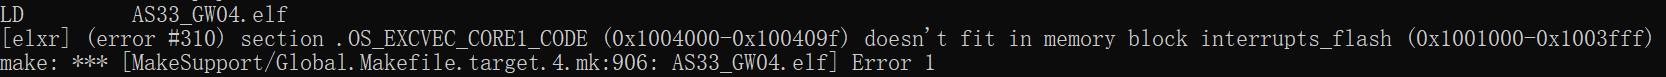
\includegraphics[scale=0.6]{pic/eth_ld_error_interrupts_flash_overflow.png}
    \caption{\lstinline{interrupts_flash flash} 块大小溢出错误}
    \label{fig:eth_ld_error_interrupts_flash_overflow}
\end{figure}

当前关于 \lstinline{interrupts_flash flash} 中存放的内容及其对齐大小如下:

\begin{lstlisting}
OS_INTVEC_CODE 32
	1024 OS_INTVEC_CODE 32
OS_INTVEC_CONST
	OS_INTVEC_CONST 32
OS_INTVEC_CORE0_CODE 1024
	4096 OS_INTVEC_CORE0_CODE 32
OS_INTVEC_CORE0_CONST 32
	4096 OS_INTVEC_CORE0_CONST 32
OS_INTVEC_CORE1_CODE 32
	4096 OS_INTVEC_CORE1_CODE 32
OS_INTVEC_CORE1_CONST 32
	4096 OS_INTVEC_CORE1_CONST 32
OS_EXCVEC_CORE0_CODE 256
	256 OS_EXCVEC_CORE0_CODE 32
OS_EXCVEC_CORE0_CONST 256
	256 OS_EXCVEC_CORE0_CONST 32	
OS_EXCVEC_CORE1_CODE 256
	256 OS_EXCVEC_CORE0_CODE 32
OS_EXCVEC_CORE1_CONST 256
	256 OS_EXCVEC_CORE0_CONST 32	
\end{lstlisting}